\section{Implementation details}
This section covers the code that performed most of the experiments used for the research in Sections 2, 5 and 6.

\subsection{Twitter Experiments}
Most processing has been done using the \textit{Ruby}\footnote{http://www.ruby-lang.org/en/}
language, a dynamic, scripting open source programming language. This allowed us
to focus on experimenting instead of implementation. The profiler scripts have been
separated from any native extensions, making them compatible with \textit{JRuby}\footnote{http://www.jruby.org} -- the Java implementation
of the Ruby language.
\subsubsection{Structure}
The Extractor part retrieves the data from Twitter. The Twitter API requests are been handled via the \textit{OAuth}\footnote{http://oauth.net/} protocol and provided in a
\textit{JSON}-based stream form. Only the newest tweets for the Twitter
users are downloaded. The entities definitions and semantics are provided by
the \textit{FreeBase} database REST interface. All further processing by the Associator
occurs locally on the pre-loaded Twitter data. \\

\begin{figure}[h!]
  \begin{center}
	  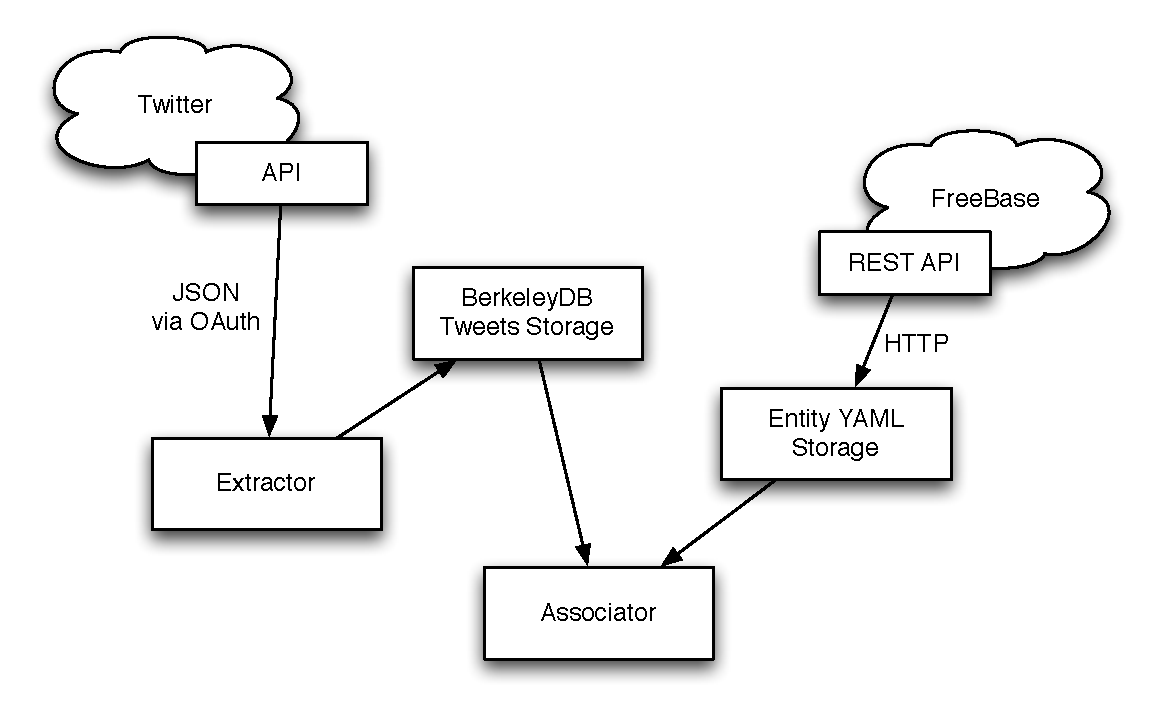
\includegraphics[scale=0.65]{images/twitter_diagram.pdf}
	  \caption{The structure of the Twitter data experiments workflow}
  \end{center}
\end{figure}

\subsubsection{Tools}
Apart from using the standard Ruby libraries, separate open-source Ruby gems have been used for the experiment:
\begin{itemize}
  \item \textit{bdb}\footnote{http://github.com/mattbauer/bdb} - a wrapper for the BerkeleyDB C driver
  \item \textit{twitter}\footnote{http://github.com/jnunemaker/twitter} - a wrapper around the Twitter API
  \item \textit{ferret} \footnote{http://ferret.davebalmain.com} - full text search engine written in pure Ruby
  \item \textit{ken}\footnote{http://github.com/michael/ken} - a wrapper for the freebase.org API
\end{itemize}

\subsubsection{Storage}
Due to Twitter API request rate limiting, tweets have been aggregated in a local
\textit{Berkeley DB} database instance providing a fast and easy key-value
information retrieval. Since a huge amount of data needs to be processed, a full
text search engine has been used, which greatly increased the searching time. In
this case, we decided on using \textit{ferret} - a full-text search engine
written in Ruby (similar to Apache's \textit{Lucene}).

\subsection{YouTube Experiments}
The code used for the research was written in \textit{Python}\footnote{http://www.python.org}
programming language. Using high-level programming language let us focus on the code itself, and skip the
gory details like memory management.

\subsubsection{Structure and Workflow}
The main program -- that's the one responsible for generating user's preferences
-- connects to \textit{YouTube} API in order to receive the required data. The
API responses come as xml documents, and are further processed and analyzed in search of
pieces of data, that are of interest to the examined subject.

\begin{figure}[h!]
  \begin{center}
	  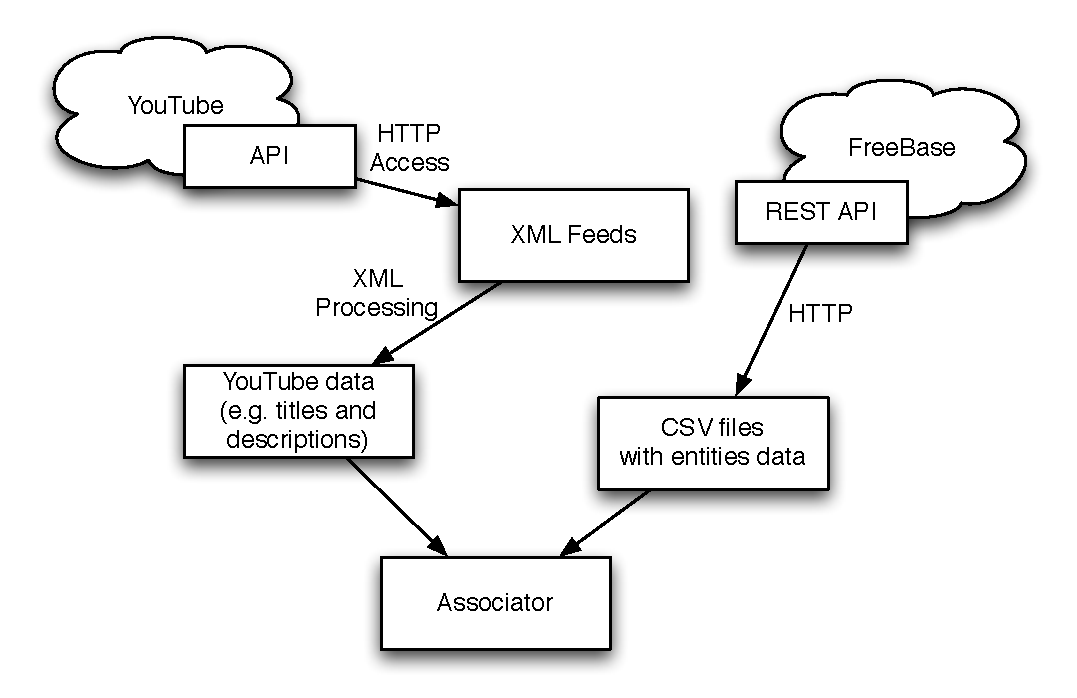
\includegraphics[scale=0.65]{images/youtube_diagram.pdf}
	  \caption{The structure of the YouTube data experiments workflow}
  \end{center}
\end{figure}

\subsubsection{Tools}

The code for user profiling depends solely on modules contained in the standard
library, which simplifies the installation process and lets us avoid dependency
on a particular Python implementation (such an approach makes the eventual
switch to \textit{Jython}\footnote{http://www.jython.org} far easier). The
standard library modules used were: ElementTree -- for xml processing, csv --
for reading freebase data dumps and urllib2 -- for accessing the API.

A set of additional scripts was prepared that were used for YouTube data
analysis. These scripts rather than analyzing single user's data, worked over a
large number of users in order to gather information on how YouTube is used.
This information includes number of people using various features (see section
3.1.1), rates of videos with identifieable linked data concepts (section 7.2).
Parts of data extracted for this research was only possible to obtain after
authentication. This was performed using http-based Google's protocol designed
for this purpose.

The corpora for analysis was collected using bfs graph traversal through YouTube
contacts. The corpus of video titles and descriptions was collected based on
those user's favourites.
